\documentclass[12pt]{article}
\usepackage[margin=2.5cm]{geometry}
\usepackage{enumerate}
\usepackage{amsfonts}
\usepackage{amsmath}
\usepackage{fancyhdr}
\usepackage{amsmath}
\usepackage{amssymb}
\usepackage{amsthm}
\usepackage{mdframed}
\usepackage{graphicx}
\usepackage{subcaption}
\usepackage{adjustbox}
\usepackage{listings}
\usepackage{xcolor}
\usepackage{booktabs}
\usepackage[utf]{kotex}
\usepackage{hyperref}

\definecolor{codegreen}{rgb}{0,0.6,0}
\definecolor{codegray}{rgb}{0.5,0.5,0.5}
\definecolor{codepurple}{rgb}{0.58,0,0.82}
\definecolor{backcolour}{rgb}{0.95,0.95,0.92}

\lstdefinestyle{mystyle}{
    backgroundcolor=\color{backcolour},
    commentstyle=\color{codegreen},
    keywordstyle=\color{magenta},
    numberstyle=\tiny\color{codegray},
    stringstyle=\color{codepurple},
    basicstyle=\ttfamily\footnotesize,
    breakatwhitespace=false,
    breaklines=true,
    captionpos=b,
    keepspaces=true,
    numbers=left,
    numbersep=5pt,
    showspaces=false,
    showstringspaces=false,
    showtabs=false,
    tabsize=1
}

\lstset{style=mystyle}

\pagestyle{fancy}
\renewcommand{\headrulewidth}{0.4pt}
\lhead{CSC 343}
\rhead{Worksheet 2 Solution}

\begin{document}
\title{CSC343 Worksheet 2 Solution}
\maketitle

\bigskip

\begin{enumerate}
    \item \textbf{Exercise 2.4.1:}

    \begin{enumerate}[a)]
        \item

        $\sigma_{speed \geq 3.0}\text{(Movies)}$

        \bigskip

        Models 1005, 1006, 1013 have speed greater than 3.0

        \bigskip

        \begin{center}
        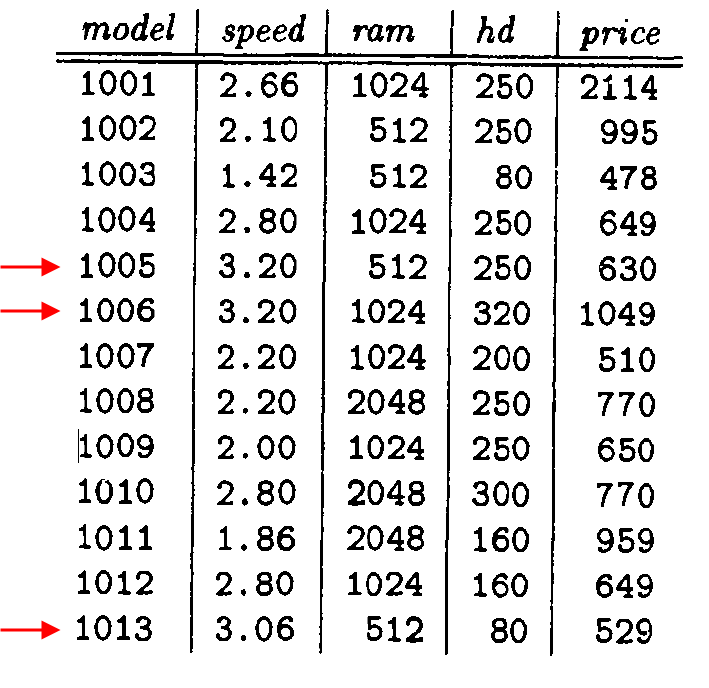
\includegraphics[width=0.4\linewidth]{images/worksheet_2_solution_2.png}
        \end{center}

        \bigskip

        \underline{\textbf{Notes:}}

        \bigskip

        \begin{itemize}
            \item Select
            \begin{itemize}
                \item Is indicated by $\sigma$
                \item \textbf{Syntax:} $\sigma_{\text{QUERY}} \text{SCHEMA\_NAME}$
                \item e.g $\sigma_{length \geq 100 \textbf{ AND } studioName=`Fox'} \text{(Movies)}$

                \bigskip

                \begin{center}
                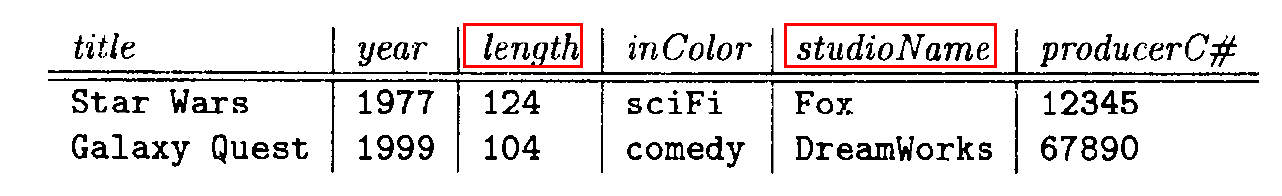
\includegraphics[width=\linewidth]{images/worksheet_2_solution_1.png}
                \end{center}
            \end{itemize}
        \end{itemize}

        \item

        $\pi_{maker}(\sigma_{hd \geq 100}(\text{Product} \bowtie \text{Laptop}))$

        \bigskip

        Makers $A,E,F,G$ make laptops with hard-disk of at least 100GB.

        \bigskip

        \begin{center}
        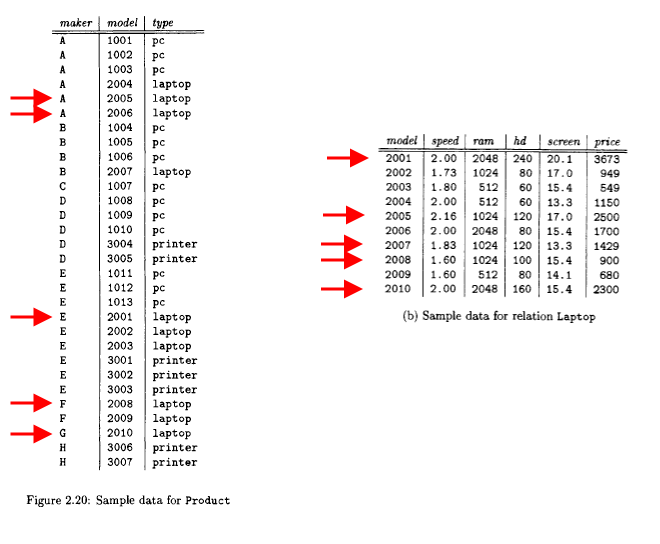
\includegraphics[width=\linewidth]{images/worksheet_2_solution_7.png}
        \end{center}

        \underline{\textbf{Notes:}}

        \bigskip

        \begin{itemize}
            \item Project
            \begin{itemize}
                \item \textbf{Syntax:} $\pi_{A_1, A_2, \cdots, A_n}$(Rel)
                \begin{itemize}
                    \item $A_1,\cdots,A_n$ represents attributes
                \end{itemize}
                \item Picks certain columns
                \item e.g

                \bigskip

                What are the titles and years of movies made by Fox that
                are at least 100 minutes long?

                \begin{align*}
                    \pi_{title,year}(\sigma_{length \geq 100 \textbf{ AND } studioName=`\textbf{Fox}'})(\text{Movies})
                \end{align*}
            \end{itemize}

            \item Cross-Product / Cartesian Product
            \begin{itemize}
                \item Combines two relations
                \item \textbf{Syntax:} Relation 1 $\times$ Relation 2
                \item e.g. Names and GPAs of students with $HS > 1000$ who applied
                to CS and were rejected

                \bigskip

                $ \pi_{sName, GPA}(\sigma_{Student.sID = Apply.sID \textbf{ AND }
                HS > 1000 \textbf{ AND } major = `cs' \textbf{ AND } dec = `R'})$(Student $\times$ Apply)

                \bigskip

                \begin{center}
                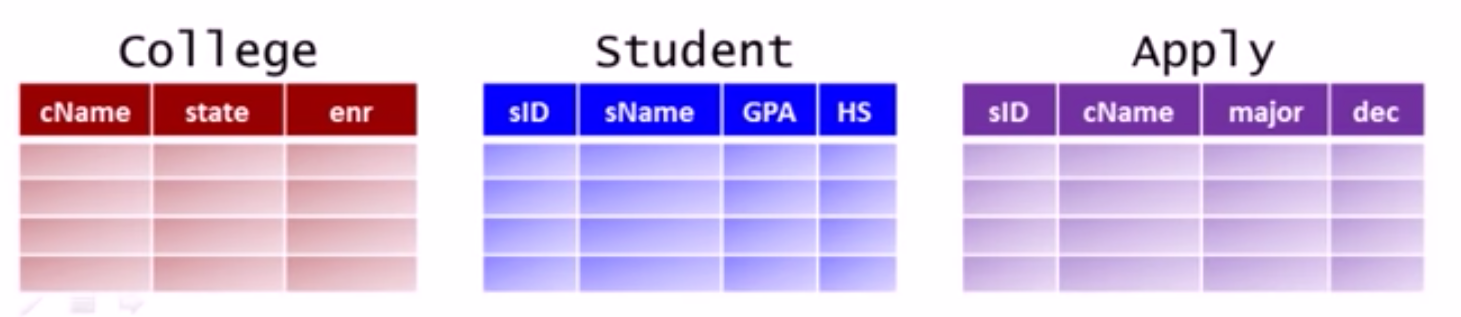
\includegraphics[width=\linewidth]{images/worksheet_2_solution_4.png}
                \end{center}
            \end{itemize}

            \item Natural Join
            \begin{itemize}
                \item Enforce equality on all attributes with the same name
                \item Eliminiate one copy of duplicate attributes
                \item Is symbolized by $\bowtie$
                \item \textbf{Syntax:} $\text{Relation 1} \bowtie \text{Relation 2}$
                \item e.g.

                \bigskip

                Names and GPAs of students with $HS > 1000$ who applied to CS and were
                rejected.

                \bigskip

                \begin{align*}
                    \pi_{sName,GPA} (\sigma_{HS > 1000 \textbf{ AND } major = `cs' \textbf{ AND } dec = `R'}\text{(Student $\bowtie$ Apply)})
                \end{align*}


                \begin{center}
                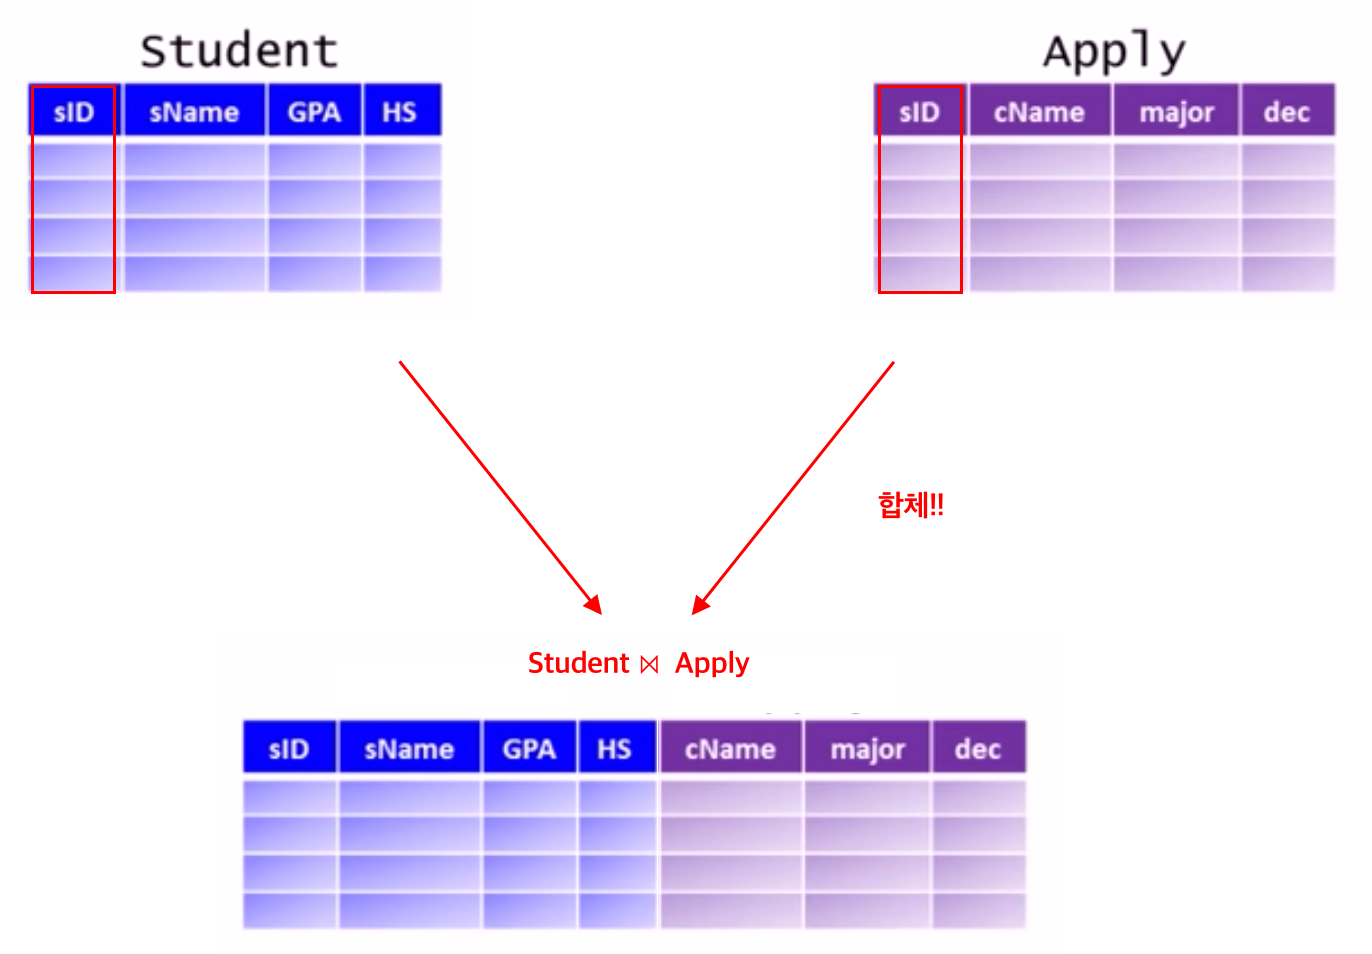
\includegraphics[width=\linewidth]{images/worksheet_2_solution_5.png}
                \end{center}

                \item e.g.2.

                \bigskip

                Names and GPAs of students with $HS > 1000$ who applied to CS
                at college with $enr > 20,000$ and were rejected

                \bigskip

                \begin{align*}
                    \begin{split}
                        &\pi_{sName,GPA} (\\
                        &\sigma_{HS > 1000 \textbf{ AND } enr > 20000 \textbf{ AND } major = `cs' \textbf{ AND } dec = `R'}\text{(Student $\bowtie$ (Apply $\bowtie$ College))}\\
                        &)
                    \end{split}
                \end{align*}

                \begin{center}
                
\includegraphics[width=\linewidth]{images/worksheet_2_solution_6.png}
                \end{center}

            \end{itemize}

            \item Union Operator
            \begin{itemize}
                \item \textbf{Syntax} $\text{R} \cup \text{S}$
                \item Is the set of elements that are in $R$ or $S$ or both.
                \item An element appears only once in the union even if it is
                    present in both $R$ and $S$.
                \item Is like \textbf{UNION} keyword in SQL
                \item e.g.

                \bigskip

                List of college and student names

                \begin{align*}
                    \pi_{cName}(\text{College}) \cup \pi_{sName} (\text{Student})
                \end{align*}
            \end{itemize}


            \item Difference Operator
            \begin{itemize}
                \item \textbf{Syntax:} $R - S$
                \item Is also called the \textit{difference} of $R$ and $S$
                \item is the set of elements that are in $R$ but not in $S$.
                \item Is like \textbf{EXCEPT} keyword in SQL
                \item e.g.

                \bigskip

                IDs and names of students who didn't apply anywhere

                \begin{align*}
                    \pi_{sID} (\text{Student}) - \pi_{sID}(\text{Apply})
                \end{align*}
            \end{itemize}

            \item Intersection Operator
            \begin{itemize}
                \item \textbf{Syntax:} $R \cap S$
                \item Is also canned the \textit{intersection} of $R$ and $S$
                \item Is the set of elements that are in both $R$ and $S$
                \item e.g.

                \bigskip

                Names that are both a college name and a student name

                \bigskip

                \begin{align*}
                    \pi_{cName} (\text{College}) - \pi_{sName}(\text{Student})
                \end{align*}
            \end{itemize}
        \end{itemize}

        \item

        \begin{align}
            \begin{split}
            &\pi_{model,price}(\sigma_{maker=`\text{B}'}(\\
            &\text{Product} \bowtie (\pi_{model,price}(\text{Laptop}) \cup \pi_{model,price}(\text{PC}) \cup \pi_{model,price}(\text{Printer})\\
            &))
            \end{split}
        \end{align}

        \bigskip

        The price and model number of all products made by manufacturer B are


        \begin{enumerate}[1.]
            \item model 1004, price 649
            \item model 1005, price 630
            \item model 1006, price 1049
            \item model 2007, price 1429
        \end{enumerate}

        \begin{center}
        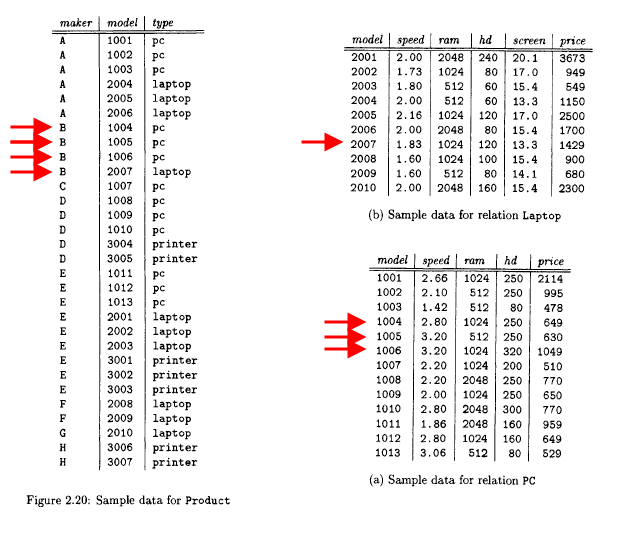
\includegraphics[width=\linewidth]{images/worksheet_2_solution_8.png}
        \end{center}


        \item $\pi_{model} (\sigma_{color = \text{true} \textbf{ AND } type=`\text{laser}'}(\text{Printer}))$

        \bigskip

        Model 3003, and 3007 are color laster printers

        \begin{center}
        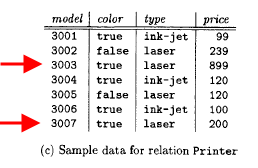
\includegraphics[width=0.4\linewidth]{images/worksheet_2_solution_9.png}
        \end{center}

        \item $\pi_{maker}(\text{Product} \bowtie (\pi_{model} (\text{Laptops}) - \pi_{model} (\text{PC})))$

        \bigskip

        Manufacturers $F$ and $G$ produce laptops but not PCs

        \begin{center}
        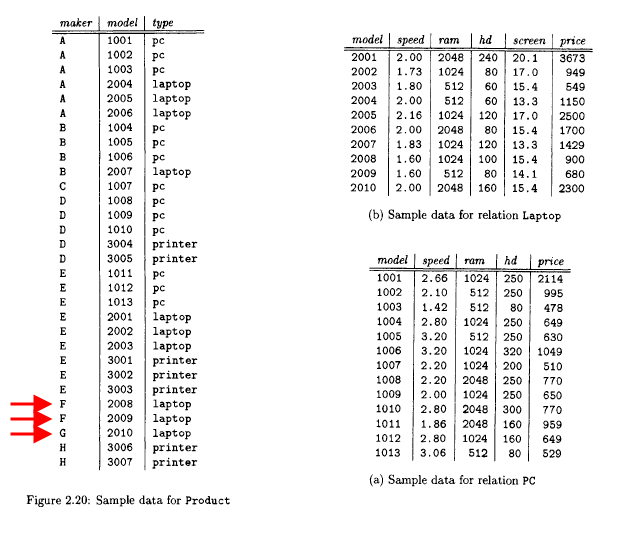
\includegraphics[width=\linewidth]{images/worksheet_2_solution_10.png}
        \end{center}

        \bigskip

        \begin{mdframed}
            \underline{\textbf{Correct Solution:}}

            \bigskip

            \color{red}

            \textbf{Relational Algebra:}

            \bigskip

            $\color{red}\pi_{maker}(\sigma_{type = `\text{laptop}' \textbf{ AND } type <> `\text{PC}'}(\text{Product}))$

            \bigskip

            \textbf{Query Result:}

            \bigskip

            \begin{tabular}{|c|}
                \hline
                maker\\
                \hline
                F\\
                \hline
                G\\
                \hline
            \end{tabular}
            \color{black}

            \bigskip

            Manufacturers $F$ and $G$ produce laptops but not PCs
        \end{mdframed}

        \bigskip

        \underline{\textbf{Notes:}}

        \bigskip

        \begin{itemize}
            \item `$<>$' Means `NOT EQUAL' in relational algebra
            \item Relational algebra inclues \underline{six} comparison operators
            ($=,<>,<,>,\geq,\leq)$ $^{[1]}$
            \item Relational projection (i.e. $\pi$) \underline{always} return
            distinct tuples $^{[2]}$
        \end{itemize}

        \bigskip

        \underline{\textbf{Reference:}}

        \bigskip

        \begin{enumerate}[1)]
            \item Radboud University: IS0 - Relational Languages, \href{http://www.cs.ru.nl/~gerp/IS0/sheets/IS0_Relationele_Algebra_SQL2.pdf}{link}
            \item Stack Overflow: Selecting DISTINCT rows in relational algebra, \href{https://stackoverflow.com/questions/4775728/selecting-distinct-rows-in-relational-algebra}{link}
        \end{enumerate}



        \item $\pi_{hd}(\sigma_{hd = hd2}(\pi_{hd}(PC) \times \rho_{\pi_{hd}(PC)(hd2)}(\pi_{hd}(PC))))$

        \bigskip

        \textbf{Query Result:}

        \bigskip

        \begin{tabular}{|c|}
            \hline
            hd\\
            \hline
            250\\
            \hline
            80\\
            \hline
            160\\
            \hline
        \end{tabular}
    \end{enumerate}

    \item

    \begin{enumerate}[a)]
        \item

        \textbf{Answer:}

        \bigskip

        \begin{center}
        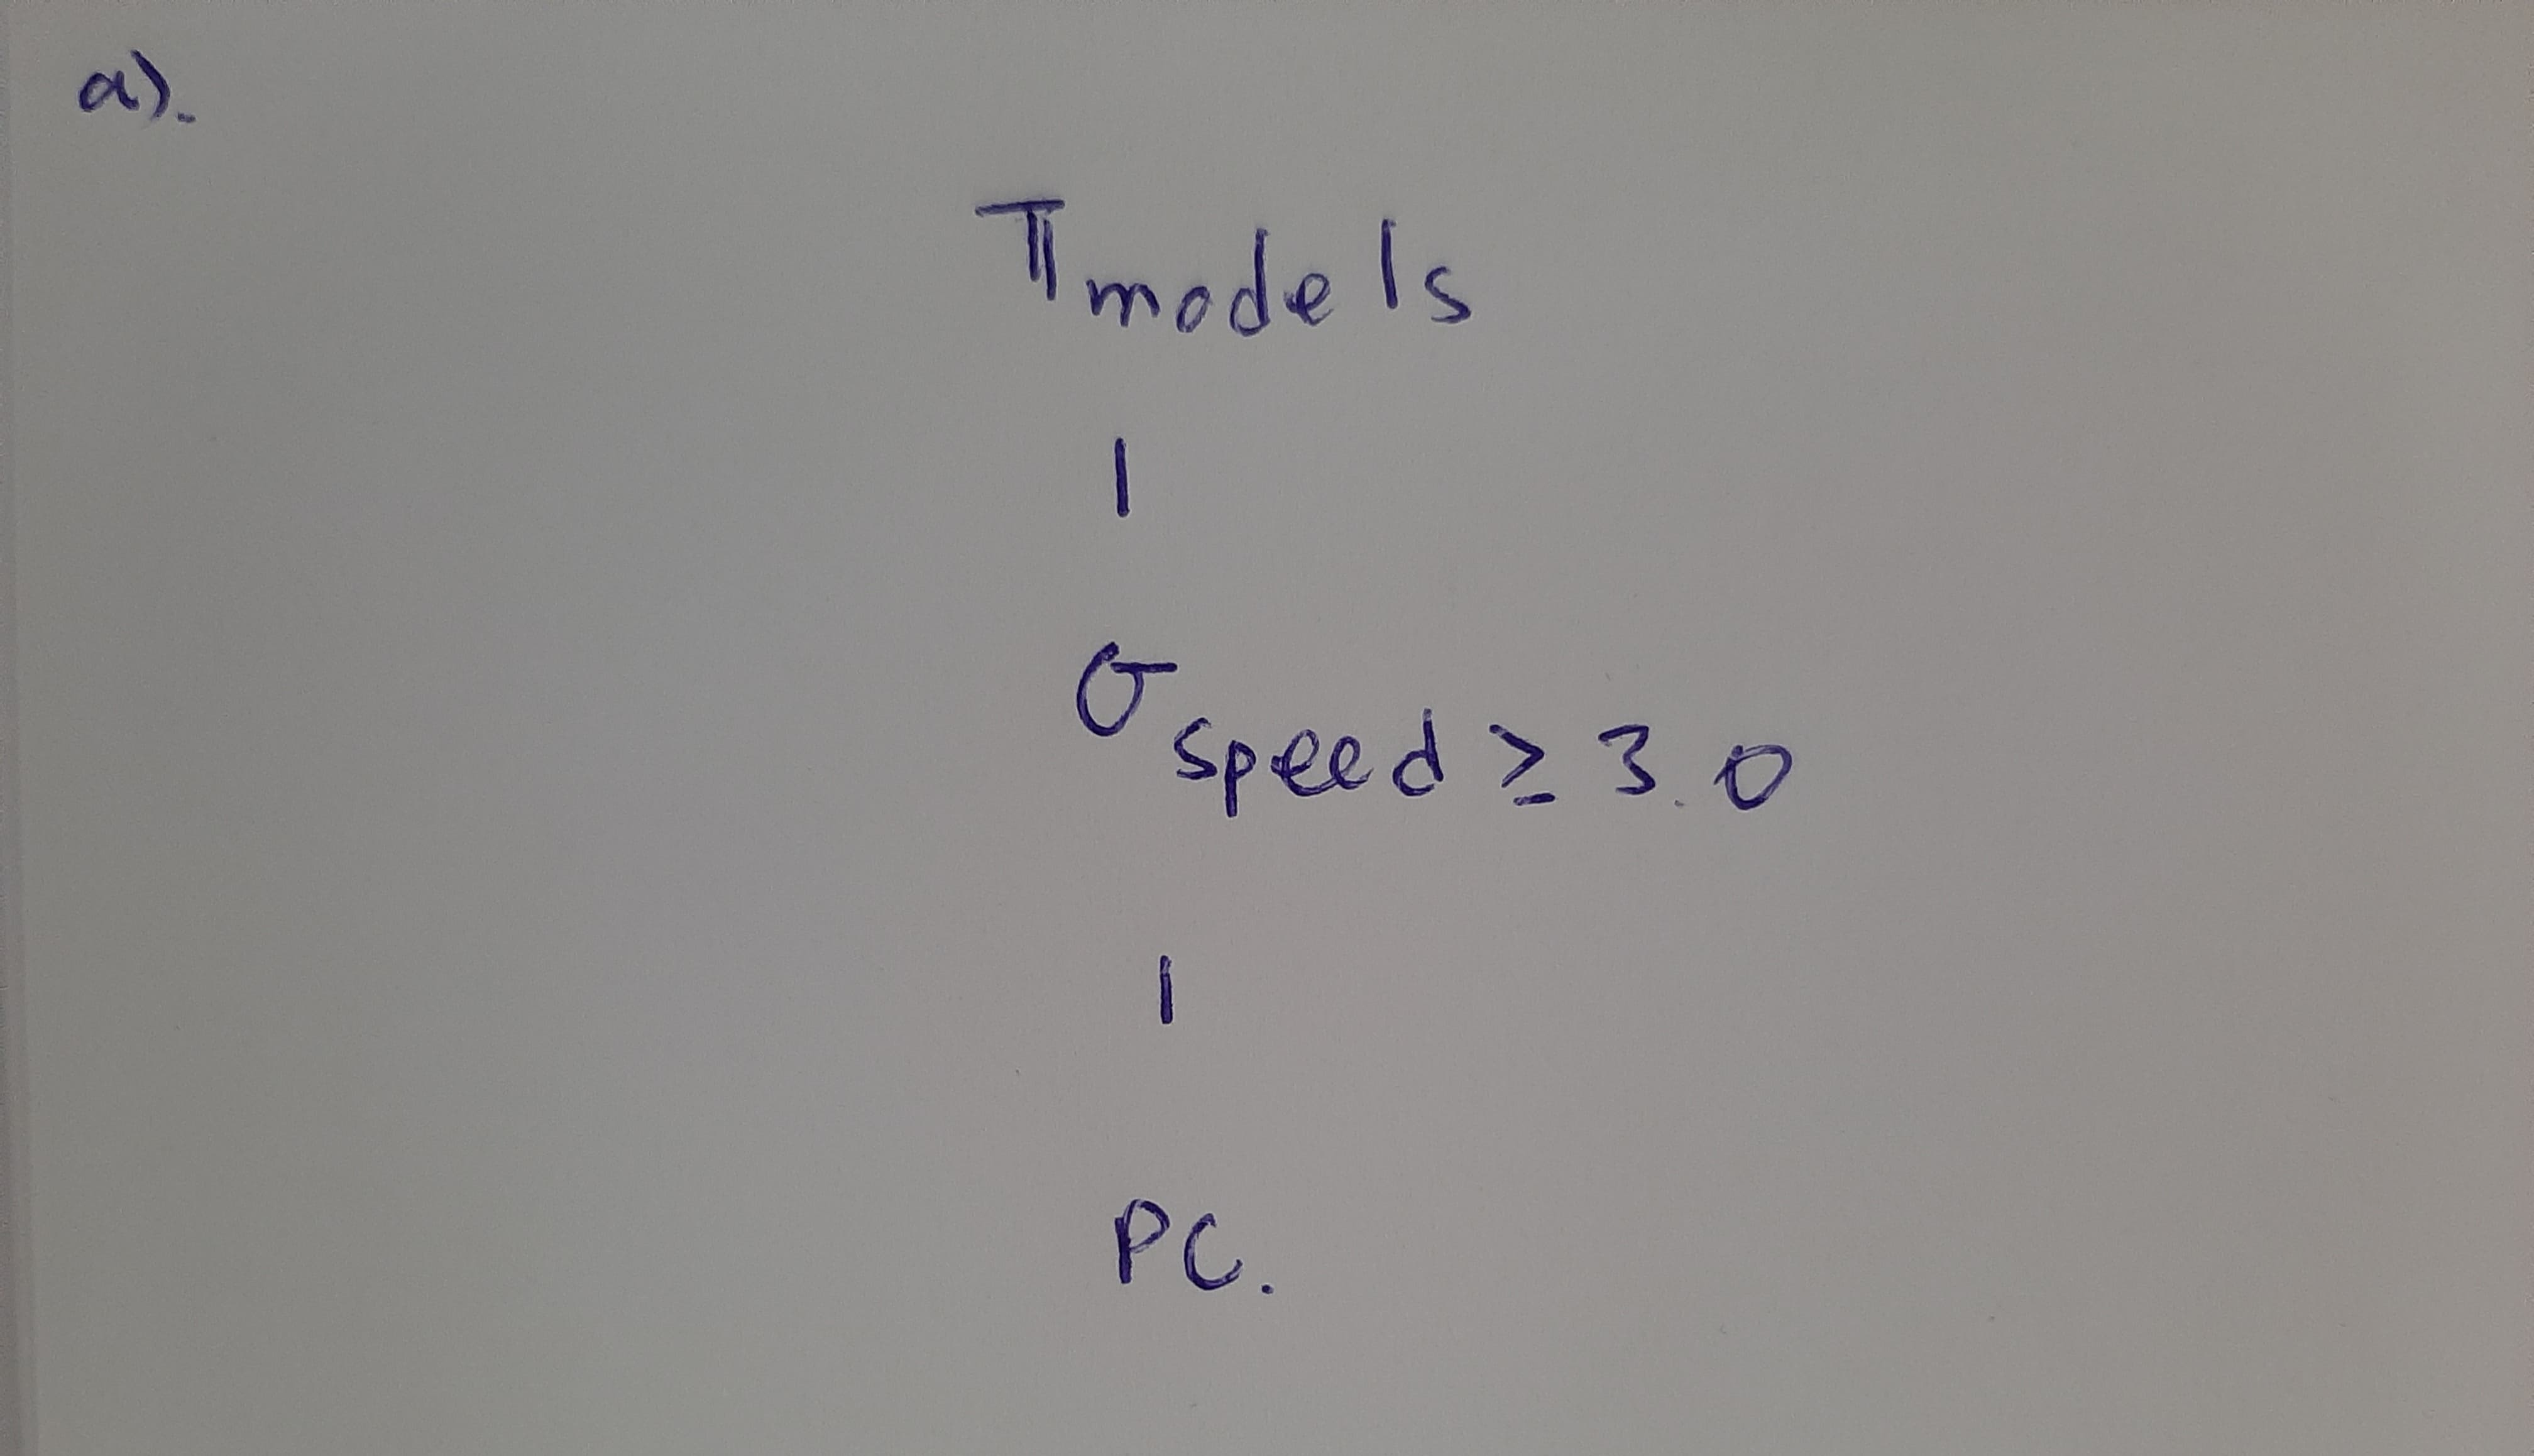
\includegraphics[width=0.7\linewidth]{images/worksheet_2_solution_11.jpg}
        \end{center}

        \item

        \textbf{Answer:}

        \bigskip

        \begin{center}
        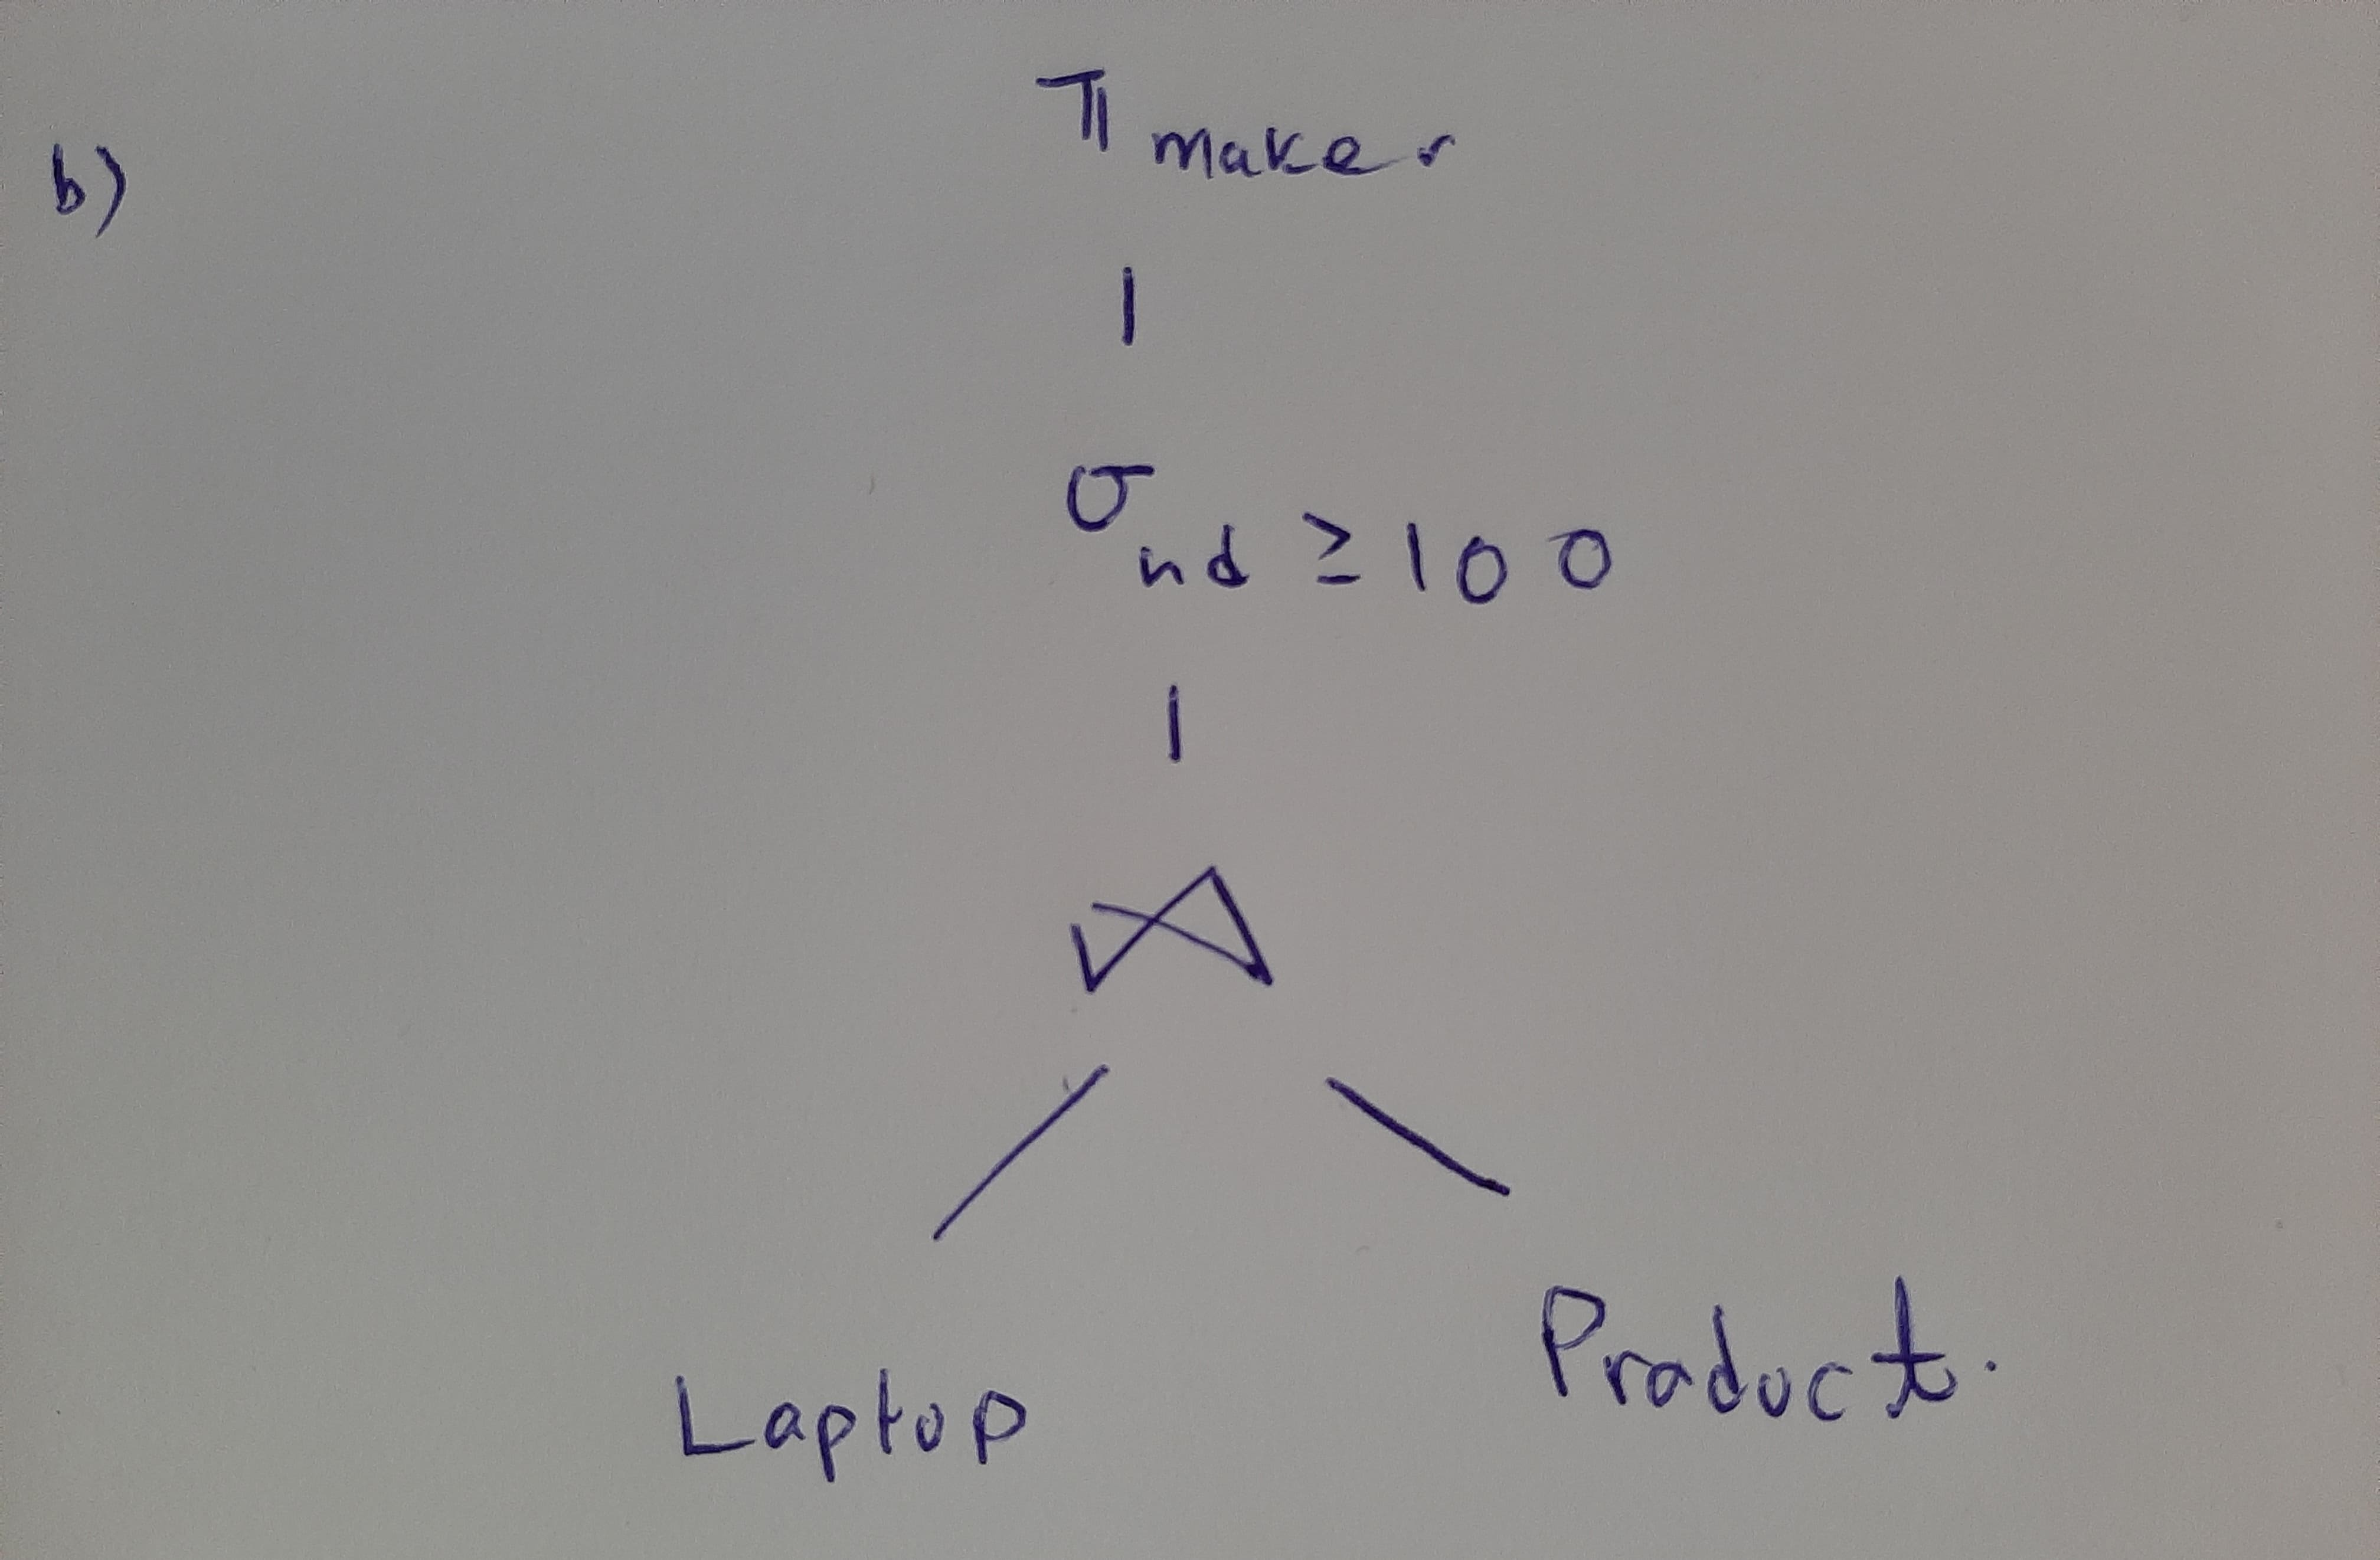
\includegraphics[width=0.7\linewidth]{images/worksheet_2_solution_12.jpg}
        \end{center}

        \item

        \textbf{Answer:}

        \bigskip

        \begin{center}
        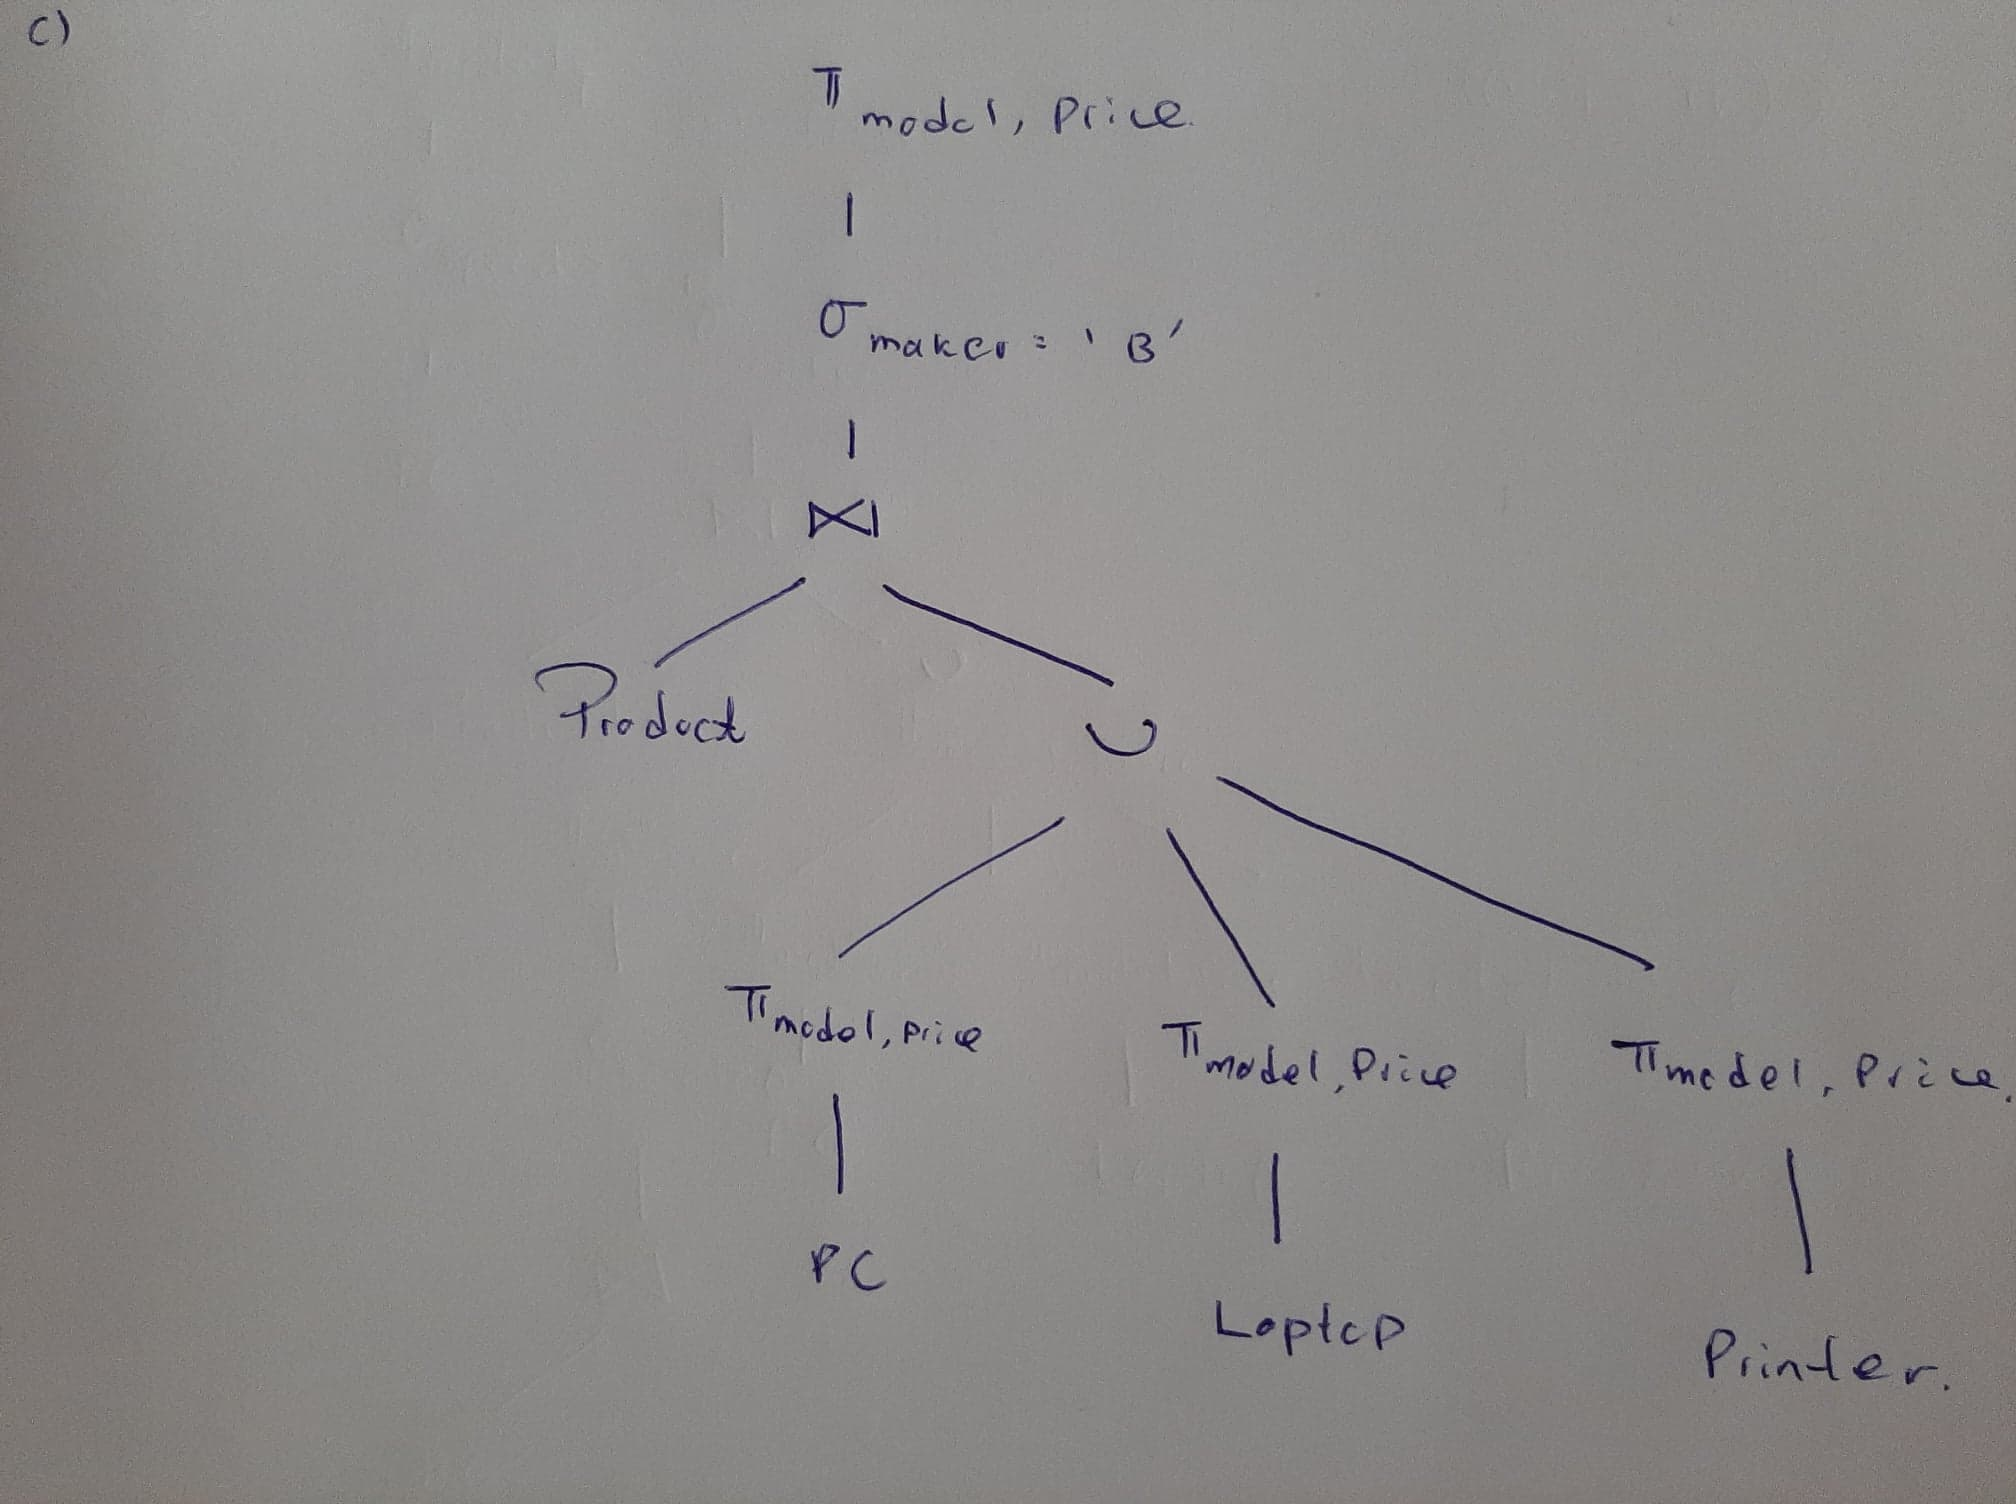
\includegraphics[width=0.7\linewidth]{images/worksheet_2_solution_13.jpg}
        \end{center}

        \item

        \textbf{Answer:}

        \bigskip

        \begin{center}
        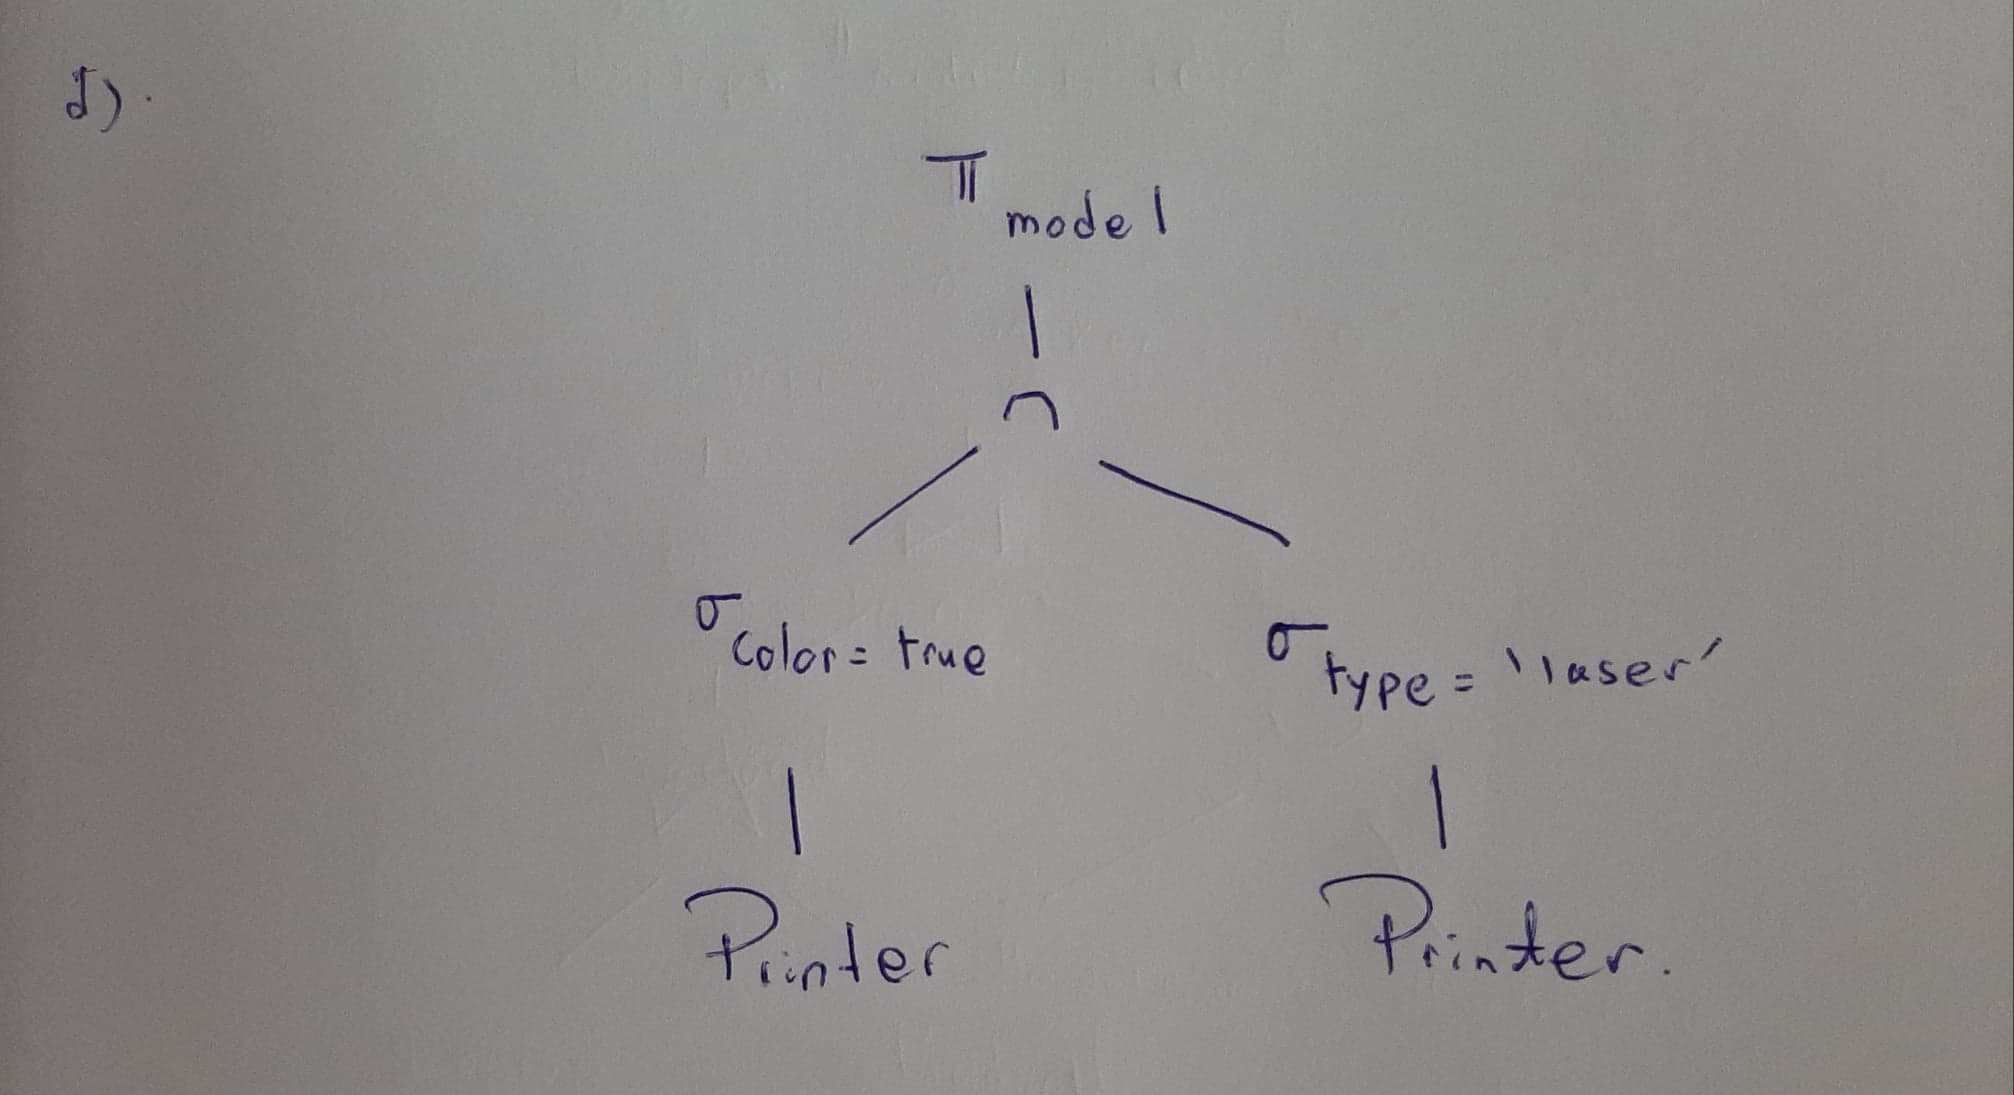
\includegraphics[width=0.7\linewidth]{images/worksheet_2_solution_14.jpg}
        \end{center}
    \end{enumerate}


\end{enumerate}

\end{document}